% !TeX TS-program = xelatex
% !Mode TeXUTF-8
%# -- codingutf-8 --
% !TeX encoding = UTF-8

%%%%%%%%%%%%%%%%%%%%%%%%%%%%%%%%%%%%%%%%
% 文件名 :     myTemplate.tex          
%                                      
% 创建:        包小敏                  
%                                      
% 创建于:      2011年02月21日          
% 最后修改于:  2024年08月16日          
%%%%%%%%%%%%%%%%%%%%%%%%%%%%%%%%%%%%%%%%
\documentclass[a4paper,
               12pt,
               oneside
]{ctexbook}
%=========IncludePackages====================
\usepackage{preample/SWUthesis}
%============================================
\makeindex % 生成索引
%=========请填入相应的内容====================
\newcommand{\university} {西南大学}          %
\newcommand{\school}     {数学与统计学院}     %
\newcommand{\daima}      {10635} % 单位代码
\newcommand{\city}       {重庆 400715}       %
\newcommand{\biaoti}{本科毕业论文~\LaTeX 模版} % 中文论文题目
\newcommand{\cobiaoti}{--- 附带简单的使用说明}   % 副标题，没有的话将“---附带简单的使用说明”删除
\newcommand{\enbiaoti}{Undergraduate Thesis {\LaTeX} Template} % 英文论文题目
\newcommand{\nianji}     {2021级}            % 年级
\newcommand{\banji} {3班}
\newcommand{\zhuanye}    {数学与应用数学（师范）} % 专业
\newcommand{\minzi}      {包小敏}               % 学生中文姓名
\newcommand{\englishname}{NAME of Student}  % 学生英文姓名
\newcommand{\zhixiedizhi}{北碚学府小区}      % 致谢词签名地址
\newcommand{\jiaoshi}    {包小敏}           % 指导教师姓名
\newcommand{\xuehao}     {222016314000000} % 学号
\newcommand{\nian}{2025}                   % 毕业年份
\newcommand{\nianxian}   {十八}    % 已使用年数(=2024-2006)
\newcommand{\kaitiriqi}  {2024年12月20日}  % 开题日期
\newcommand{\tijiaoriqi} {\today} % 提交日期---致谢词签名日期
\newcommand{\dayinriqi}{2025年5月} % 打印日期-封面最下方的日期
\newcommand{\dabianriqi} {2025年5月8日} 
%====================================================
% 若修改过程中某个文件不需修改，则将\includeonly中这个文件
% 名注释掉可以加快编译速度。
%
% 请用XELATEX编译!
%====================================================
\includeonly{preample/coverpage,
	         declaration/declare,
	         fujian/abstract,
	         fujian/zhixie,
	         fujian/fulu,
	         zhengwen/chaptone,
	         zhengwen/chapttwo,
	         zhengwen/chaptthree,
	         zhengwen/chaptfour,
	         zhengwen/chaptfive,
	         wenxian/bibfile
}
%====================================================
\makeindex

\begin{document}
\begin{titlepage}
% !TeX TS-program = xelatex
% !Mode TeXUTF-8
%# -- codingutf-8 --
% !TeX encoding = UTF-8
%%%%%%%%%%%%%%%%%%%%%%%%%%%%%%%%%%%%%%%%%%
\begin{center}
%要学校的logo时使用此封面头
\begin{tabu}to \linewidth{X[l]X[r]}
  \hspace{8mm}
\includegraphics[width=4cm]{preample/xidalogo.png}
        &  \raisebox{18.6ex}[0pt]{\zihao{4}{单位代码：\daima}}
\end{tabu}
\begin{tabu}to \linewidth{X[c]}
  \hspace{8mm}
\includegraphics[height=2cm,angle=0]{preample/xishi.png}\\[3pt]
  \hspace{8mm}{\bf\zihao{0}\youyuan 本科毕业论文（设计）}
\end{tabu}
%不要学校的logo时使用下面的封面头
%\begin{tabular}{c}
%
\includegraphics[height=2cm,angle=0]{preample/xishi}\\[12pt]
%
%\hspace{.8cm}{\bf\zihao{0}\youyuan 本科毕业论文（设计）}
%\end{tabular}
%-------------------------------------------------
\end{center}
\vspace{0.2cm}

\zihao{2}
\begin{center}
\tabulinesep=2mm
\begin{tabu}{X[c]}
{\songti\biaoti} \\
\end{tabu}
\end{center}
\vspace{.2cm}

\begin{center}
\begin{tabu}to 0.8\linewidth{X[c]X[c,1.8]}
	{\zihao{-2}\bf{\ziju{3.5}学院}} & {\zihao{-2}{\kaishu\school}}   \\\tabucline{2-2}
	{\zihao{-2}\bf{\ziju{3.5}专业}} & {\zihao{-2}{\kaishu\zhuanye}} \\\tabucline{2-2}
%	{\zihao{-2}\bf{\ziju{3.5}年级}} & {\zihao{-2}\kaishu\nianji\banji}     \\\tabucline{2-2}
    {\zihao{-2}\bf{\ziju{3.5}姓名}} & {\zihao{-2}\kaishu\minzi}      \\\tabucline{2-2}
	{\zihao{-2}\bf{\ziju{3.5}学号}} & {\zihao{-2}\xuehao}            \\\tabucline{2-2}
	{\zihao{-2}\bf{\ziju{0.5}指导教师}} & {\zihao{-2}\kaishu\jiaoshi}    \\\tabucline{2-2}
	{\zihao{-2}\bf{\ziju{0.5}答辩日期}} & {\zihao{-2}{\kaishu\dabianriqi}} 
	\\\tabucline{2-2}
\end{tabu}
\vspace{2.8cm}

{\zihao{3}\youyuan{\dayinriqi}}
\end{center}

\end{titlepage}
%==================原 创 声 明======================
\thispagestyle{empty}%
\pagenumbering{roman}%
% !TeX TS-program = xelatex
% !Mode TeXUTF-8
%# -- codingutf-8 --
% !TeX encoding = UTF-8
%%%%%%%%%%%%%%%%%%%%%%%%%%%%%
\addcontentsline{toc}{chapter}{独创声明}
%\thispagestyle{empty}
\centerline{\zihao{3}\bf 独创声明}
\vspace{1cm}

{\zihao{4}

本人郑重声明：所呈交的毕业论文（设计），是本人在指导老师的指导下，独立进行研究工作所取得的成果，成果不存在知识产权争议。尽我所知，除文中已经注明引用的内容外，本论文（设计）不含任何其他个人或集体已经发表或撰写过的作品成果。对本文的研究做出重要贡献的个人和集体均已在文中以明确方式标明。

声明的法律后果由本人承担。

\vspace{1.8cm}

\begin{tabu}to 0.9\linewidth{XX[r]X[l,1.4]}
	& 作者签名： & \\\cline{3-3}\\[-3pt]
    &           & \hspace{1.2cm} 年\hspace{0.8cm}月\hspace{0.8cm}日 \\
	
\end{tabu}

\vspace{1.3cm}

\begin{center}
    {\zihao{3}\bf 毕业论文（设计）使用授权声明}
\end{center}
\vspace{.5cm} 

\songti

本人完全了解西南大学关于收集、保存、使用毕业论文（设计）的规定。

本人愿意按照学校要求提交论文（设计）的印刷本和电子版，同意学校保存论文（设计）的印刷本和电子版，或采用影印、数字化或其它复制手段保存论文（设计）；同意学校在不以营利为目的的前提下，建立目录检索与阅览服务系统，公布论文（设计）的部分或全部内容，允许他人依法合理使用。

（保密论文在解密后遵守此规定）

\vspace{1.6cm}

\begin{tabu}to 0.9\linewidth{XX[r]X[l,1.4]}
	& 作者签名： & \\\cline{3-3}\\[-3pt]
	&           & \hspace{1.2cm} 年\hspace{0.8cm}月\hspace{0.8cm}日 \\
	
\end{tabu}
}


%====================目 录=========================
\pagestyle{plain}%
\tableofcontents
\newpage
%=================================================
\pagenumbering{arabic} %
\setcounter{page}{1}   %
%====================摘要==========================
% !TeX TS-program = xelatex
% !Mode TeXUTF-8
%# -- codingutf-8 --
% !TeX encoding = UTF-8
%%%%%%%%%%%%%%%%%%%%%%%%%%%%%%%%%%%%%%%%%%
\begin{center}
{\bf\zihao{3}{\biaoti}}\\[3pt]
{\zihao{-4}\cobiaoti}

\vspace{0.3cm}
{\zihao{-4}\kaishu\minzi}

{\zihao{5}\university\school，\city}
\end{center}
\addcontentsline{toc}{chapter}{摘要}
%\begin{center}
%\begin{minipage}[t]{13cm}
\noindent{\zihao{5}{\bf 摘要：}}
%--------------------------------------------------
{\fangsong
\zihao{5}
% 请填入中文摘要：
本模版是为{\university\school}本科毕业生而设计的(当然其他学院的学生也可以使用). 
模版根据{\university}论文的Word模版中所描述的要求编写~\cite{moban_wenjian,moban_fujian}. 目的是简化和
规范学位论文的撰写，使得论文作者可以将精力集中到论文的内容上而不是浪费在版面设置上.
使用者只需了解{\LaTeX}的基本概念即可使用本模版.

}\vspace{0.1cm}

\noindent{\songti\zihao{5}{\bf 关键词：} \LaTeX;模版; 论文; 版面; 参数
%---------------------------------------------------
}
\vspace{0.6cm}
%\end{minipage}
%\end{center}
\setmainfont{Times New Roman}%英文摘要用Times New Roman
\begin{center}
{\bf\zihao{4}\enbiaoti}

\vspace{0.3cm}
{\zihao{5}\englishname}

{\zihao{-5} School of Mathematics \& Statistics， Southwest University，Chongqing 400715}
\end{center}
\addcontentsline{toc}{chapter}{Abstract}
\noindent{\zihao{5}{\bf Abstract：}}
%%%%%%%%%%%%%%%%%%%%%%%%%%%%%%%%%%%%%%%%%%%%%%%%%%%%
{\zihao{5}
% 请填入英文摘要：
This \LaTeX template is designed for undergraduate students from the School of Mathematics and Statistics of Southwest University. The template is written according to the requirements described in the Word template of the School of Mathematics and Statistics. The purpose is to simplify and standardize the writing of the thesis, and allows the students to focus their energy on the content of the paper rather than wasting it on formatting. Only basic knowledge of the \LaTeX is required to use this template.

\vspace{0.1cm}
}
\noindent{\zihao{5}{\bf Key words：} \LaTeX; template; thesis; layout; parameters
%-----------------------------------------
}

%\zihao{-4}
%==================正文开始========================
% !TeX TS-program = xelatex
% !Mode TeXUTF-8
%# -- codingutf-8 --
% !TeX encoding = UTF-8
%%%%%%%%%%%%%%%%%%%%%%%%%%%%%%%%%%%%%%%
\zihao{-4}
%---------------------------------------
\chapter{关于模板的一些说明}%\label{chpt:1}
%---------------------------------------
本模版\glossary{模板}是为{\university\school}本科毕业生撰写毕业论文而设计的，版面尺寸按照{\university}的论文撰写要求选取~\cite{moban_fujian}。模板的第一版是
2006年完成的，经过多年的使用、 改进，最终发展成目前的版本。

模板的最近一次修改是2024年8月。 这次修改的变动比较大，首先 \university 对论文的结构、格式和要求进行了比较大的改动~\cite{moban_wenjian,moban_fujian}；其次，为了适应更多的使用者，本次模板的编译采用的是 XeLatex，不是以前的 PdfLatex。

第一次使用本模版时，请先阅读~\ref{subsec:1}节；%如果安装\CTeX{}\index{\CTeX} 有问题，请阅读~\ref{sec:versionSelect}节；
如果对数学公式、符号或定义、定理、证明等各种命令环境不熟悉，请阅读第~\ref{sec:2two}
节；如果对表格或图形的\index{图形插入}插入不熟悉，请阅读第~\ref{sec:ssss} 节；如果对\index{交叉引用}交叉引用不熟悉，请阅读第~\ref{sec_si4}节。 如果想了解在~\LaTeX 中\index{程序引入}引入程序代码，如
~{\tt Matlab}\index{Matlab}，{\tt Mathematica}\index{Mathematica}, {\tt Python}\index{Python}，{\tt R}\index{R} 和~{\tt C/C++}\index{C/C++} 等的代码，请阅读第~\ref{sec:codeinludsion}节, 并分别参考附录~\ref{appendix:A}、\ref{appendix:B}、\ref{appendix:E}、\ref{appendix:C}、\ref{appendix:D} 中的实例. 
\section{模板的构成}\label{subsec:1}
本模板由若干文件组成，所有文件都存放在一个主文件夹\index{文件夹}里。为了使用和管理方便，在主文件夹中又分了七个子文件夹：{\tt preample, codes, tables，declaration，zhengwen, fujian, wenxian}，其中~{\tt preample\index{文件夹!preample}, tables\index{文件夹!table}, declaration\index{文件夹!declaration}} 中的文件一般不用管。子文件夹~{\tt codes} 中放有一些制作本说明时的附件所用的一些代码文件，如果不需要可以删除。
%而~{\tt codes\index{文件夹!codes}} 在熟悉模板后可以删除。文件夹~{\tt fujian\index{文件夹!fujian}} 包含中英文摘要及附录，文件夹~{\tt declaration\index{文件夹!declaration}} 中是独创性声明，而文件夹~{\tt wenxian\index{文件夹!wenxian}} 则包含一个参考文献列表文件。模板由主文件~{\tt mytemplate.tex\index{mytemplate.tex}} 及五类子文件构成：
\begin{description}
  \item[主文件~mytemplate:] 论文的编译一般通过主文件进行。学生的基本信息，如姓名，学号，论文题目等，都在主文件上输入。主文件名可根据自己的需求改动。
  \item[文件夹~codes:]\label{item:codes} 文件夹中包含几个程序代码。如果使用者自己没有代码，可以将其删除。
  \item[文件夹~zhengwen:] 文件夹中包含五个文件，分别对应五章。使用者可以根据自己论文的实际章数来增加或减少这里的文件数，同时录入自己论文相应章节的内容。
  \item[文件夹~fujian:] 文件夹中包含以下几个文件：
  \begin{enumerate}
  	\item {\tt abstract.tex\index{abstract.tex}}，这是论文的摘要。
  	\item {\tt thanks.tex\index{thanks.tex}}，这是论文的致谢词部分。
  	\item {\tt fulu\index{文件夹!fulu.tex}}, 这是论文附录的引入文件。使用者如果没有附录，那就将附录文件~{\tt fulu}删除。
  \end{enumerate}
  \item[文件夹~wenxian:]文件夹中包含一个文件，其中是论文中所引用的参考文献。
\end{description}
%  \item\label{item:2} 这一类文件是论文的主要组成部分，由学生完成。有以下几个文件：
%  \begin{enumerate}
%    \item {\tt abstract.tex\index{abstract.tex}}，这是论文的摘要。
%    \item {\tt body.tex\index{body.tex}}，这是论文的正文部分。
%    \item {\tt bibfile.tex\index{bibfile.tex}}，这是论文的参考文献。
%    \item {\tt thanks.tex\index{thanks.tex}}，这是论文的致谢词部分。
%  \end{enumerate}
%  以上两类文件都存放在主文件夹里，学生只须在相关的文件中按~\LaTeX\index{\LaTeX} 的要求及文件中的提示输入相应的内容即可。
%  \item 这一类是三个与教师有关的文件：
%  \begin{enumerate}
%    \item\label{term1} {\tt zhidaojiaoshigeifen.sty}，这个文件包含指导教师评分及评阅意见，由指导教师完成。
%    \item {\tt jiaochageifen.sty}，这个文件包含交叉评阅意见及评分，由负责交叉评阅的教师完成。
%    \item {\tt dabianchengji.sty}，这个文件包含答辩评审意见、答辩分数及论文成绩，由教师答辩小组组长完成。
%  \end{enumerate}
%  这类文件存放在子文件夹~{\tt filesforteachers} 中。相关教师只须在对应的文件中按\LaTeX
%  的要求及文件中的提示输入相应的内容即可。具体的对应文件及填写方法参看后面表格(开题报告二，教师评阅表，交叉评阅表，答辩记录表)中的说明。
%  \item 这一类有两个个文件：
%  \begin{enumerate}
%    \item {\tt kaitibaogao.tex}（开题报告）；
%    \item {\tt dabianjilu.tex\index{dabianjilu.tex}}（答辩记录）。
%  \end{enumerate}
%   这类文件存放在子文件夹~{\tt filesforstudent} 中。第一个文件用来填写开题报告的具体内容，后一个文件是用来填写答辩的记录内容。完成人只须在对应的文件中按~\LaTeX 的要求及文件中的提示输入相应的内容即可。
%   具体的对应文件及填写方法参看后面表格（开题报告一，第开题报告二，答辩记录表）中的说明。
%  \item\label{item:4} 这一类是三个与教师有关的文件：
%  \begin{description}
%    \item\label{term1} {\tt zhidaojiaoshigeifen.tex\index{zhidaojiaoshigeifen.tex}}，这个文件包含指导教师评分及评阅意见，由指导教师完成。
%    \item {\tt jiaochageifen.tex\index{jiaochageifen.tex}}，这个文件包含交叉评阅意见及评分，由负责交叉评阅的教师完成。
%    \item {\tt dabianchengji.tex\index{dabianchengji.tex}}，这个文件包含答辩评审意见及论文评定成绩，由教师答辩小组组长完成。
%  \end{description}
%  这类文件存放在子文件夹~{\tt filesforteachers} 中。具体操作时，学生可以将相关的文件发给相关教师，相关教师只须在对应的文件中按~\LaTeX
%  的要求及文件中的提示输入相应的内容，然后发还给学生，学生用其替换原来的同名文件再通过主文件编译即可。具体的对应文件及填写方法参看后面表格（开题报告二，指导教师评阅表，交叉评阅表，答辩记录表）中的说明。
%  \item\label{item:head} 这一类中除头文件{ \tt SWUthesis.sty\index{SWUthesis.sty}} 外还有一些诸如学校的~logo 和学院的~logo 之类的文件。
%        这几个文件单独放在子文件夹~{\tt preample} 中，这些文件一般不用改动。
%
%      这四类文件在前面相关的内容录入后，通过编译主文件，会自动将指导教师评阅意见，交叉评阅意见以及答辩记录，答辩分数和论文等级等相关的内容导入对应表格，最后生成~PDF 格式的文件。
%  \item\label{item:miscellanceous} 这一类中有六个文件：{\tt coverpage.tex\index{coverpage.tex}}（封面），
%  {\tt kaiti\_1.tex\index{kaiti\_1.tex}}（开题报告表格的前半部分），{\tt kaiti\_2.tex\index{kaiti\_2.tex}} （开题报告表格的后半部分），
%  {\tt pingyue\_1.tex\index{pingyue\_1.tex}}（指导教师评阅表）， {\tt pingyue\_2.tex\index{pingyue\_2.tex}} （交叉评阅表），
%        {\tt dabian.tex}（答辩记录表）。这几个文件，单独放在子文件夹~{\tt tables} 中，它们只生成封面或表格的框架，其中需要填入的内容通过编译会自动从其它相关文件中导入，
%        所以一般不用对这些文件做改动。
%\end{enumerate}
%总之第~\ref{item:head} 类和第~\ref{item:miscellanceous} 类的文件一般不用去管，主文件和~\ref{item:2}--~\ref{item:4} 类中的子文件在完成后由学生统一通过主文件编译，
%最后生成包含所有内容和所有表格的、完整的论文的~PDF 格式的文件。子文件夹~{\tt codes} 中放有一些制作本说明时所用的一些文件，如果不需要可以删除。
\subsection{三级标题}
\fbox{本节为测试三级标题在目录中的显示而设。}
\section{\TeX 简介\index{\TeX}}
\TeX 是计算机科学家、图灵奖\index{图灵奖}得主~Knuth\index{Knuth} 教授设计的一款权威的科技论文排版软件！学习~\TeX(\LaTeX)，
Knuth 的专著~\cite{knuth} 无疑是权威之选。该书排版堪称完美，从中可以看出大师的魅力。更重要的是~Knuth 教授无偿公开了~\TeX{} 的所有源代码，
也就是说它是开源 (Open Source)的（通俗地说就是可以免费使用）。正因为这个原因，后人在其基础上开发了~\LaTeX 。\LaTeX 方便好用，被广泛传播，成了当今世界科技界最权威的论文排版软件。
作为一个非常全面的~\LaTeX{} 的参考书，\cite{companion} 是一个不错的选择。如果阅读英文有困难，作为一个初学者，也可以先看看~\cite{zhanglibo}。

\TeX{} 和~\LaTeX{} 排版软件和~MS 的~Word \index{Word}软件不同，后者是``所见即所得\index{所见即所得}"(WYSIWYG\index{WYSIWYG}，what you see is what you get)，而前者是``所想即所得\index{所想即所得}"(WYWIWYG\index{WYWIWYG}，what you want is what you get)。
二者在风格上迥然不同，因此学习~\LaTeX{} 需要稍微改变一下自己的习惯。

%\paragraph{Run-in headings.}
国内较早使用的~\LaTeX 汉化版\index{\LaTeX 汉化版}是~
\CTeX，可在~\href{http://www.ctex.org}{\CTeX{} 网站}~\index{\CTeX 网站}免费下载安装。\CTeX{} 安装包自带了一个编辑器~WinEdt\index{WinEdt}, 不过这个编辑器需要注册；否则会频繁跳出弹窗，提示你注册，很是烦人！可以用~\href{https://texstudio.sourceforge.net/}{TeXstudio} \index{TeXstudio} 作为编辑器来替代~WinEdt。这时需要将~TeXstudio 和\CTeX 的编译器关联起来，当然也可以选择 TexLive + TeXstudio 的组合。TexLive\index{TexLive} 可以从清华大学的~\href{https://mirrors.tuna.tsinghua.edu.cn/CTAN/systems/texlive/Images/}{镜像网站}下载。

%---------------------------------------
\section{\LaTeX{} 文件的编译\index{\LaTeX 文件的编译}}
%---------------------------------------
\LaTeX{}的编译器\index{编译器}有多个，为了避免不必要的麻烦，本模板的编译指定采用~{\tt XeLatex}\index{XeLatex}. 因此用其它编译器编译就会报错. 另外，源文件如果是用其它编辑器录入的, 在用~TeXsdudio 打开保存之前请确认其是采用的是~UTF-8 \index{UTF-8}汉字编码\index{汉字编码}，否则文件可能会出现乱码. 可以先用记事本\index{记事本}将文件打开, 点击``文件", 在下拉菜单中选择``另存为"后会弹出一个如图~\ref{fig:ansi2utf8} 的窗口，在其下部``编码"的下拉窗口中选择``UTF-8", 然后点击保存既可转成UTF-8的编码.
\begin{figure}[ht]
  \centering
  % Requires \usepackage{graphicx}
  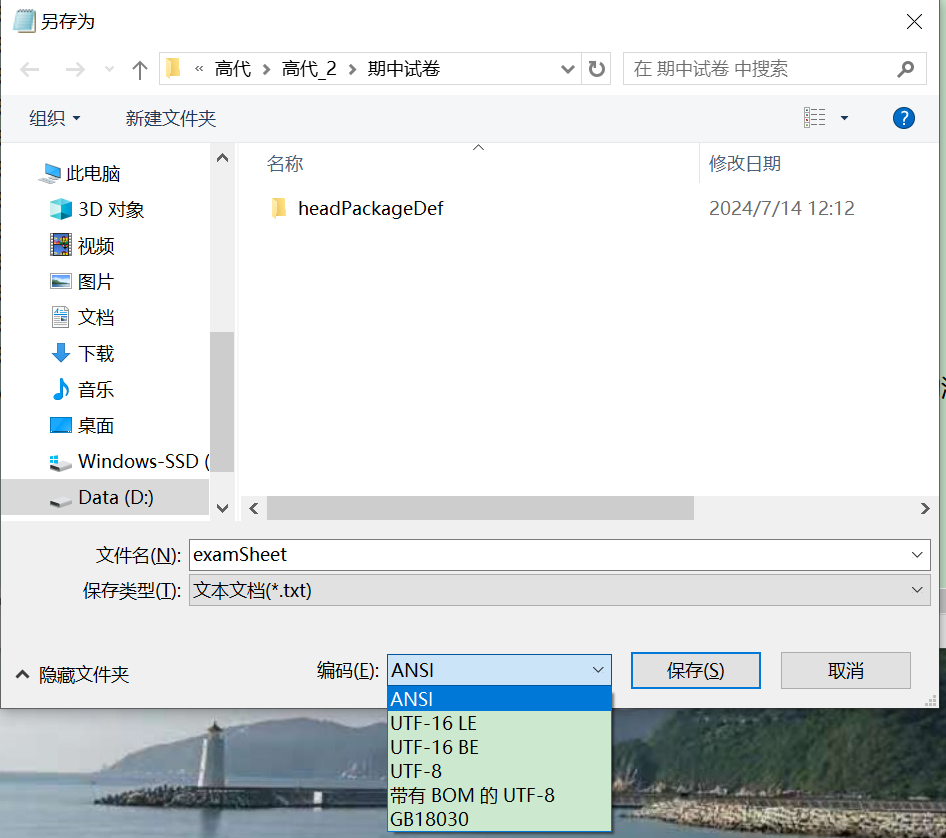
\includegraphics[width=12cm]{figs/ansi2utf8.png}\\
  \caption{ANSI编码转UTF-8编码}\label{fig:ansi2utf8}
\end{figure}

% !TeX TS-program = xelatex
% !Mode TeXUTF-8
%# -- codingutf-8 --
% !TeX encoding = UTF-8
%%%%%%%%%%%%%%%%%%%%%%%%%%%%%%%%%%%%%%%%%%

\large\zihao{-4}
%---------------------------------------
\chapter{正定矩阵及其性质}\label{sec:2two}
%---------------------------------------
\section{预备知识}
\begin{definition}
设$A\in \mathbb{R}^{n\times n}$,若$A=A^T$,对任意的$0\neq x \in \mathbb{R}^{n\times 1}$,的、均有$x^{T}Ax>0$,则称$A$为实对称正定矩阵。
\end{definition}
\begin{lemma}

\end{lemma}
\section{正定矩阵的性质}

\LaTeX 文件的输入要涉及到一些 \LaTeX 命令，尤其是数学符号和公式的输入。这里通过实例来说明如何输入一些与数学有关的内容。建议学生在使用前阅读一遍。通过对比PDF文件中的效果和源文件对应的排版命令，初学者可以快速上手使用\LaTeX 。
\begin{definition}
设
\begin{equation}\label{eq:1}
    a_1,a_2,\cdots, a_n, \cdots
\end{equation}
是一个数列。称
$$\sum_{i=1}^n a_i$$
为数列~\eqref{eq:1} 的前$n$项和\index{前$n$项和}。
\end{definition}
\begin{lemma}[新定理]
若$p$是一个素数，且$p$不能够被$a\in \mathbb{N}$整除，则
$$a^{p-1}\equiv 1\pmod{p}.$$
\end{lemma}
\begin{proof}
引理的证明在此给出。
\end{proof}
\begin{theorem}[欧拉定理\index{欧拉定理}]\label{thm:euola}
若$\gcd(a,n) = 1$，则
$$a^{\phi(n)}\equiv 1\pmod{n}.$$
\end{theorem}
\begin{proof}
下面我们来证明这个定理。
\end{proof}
\begin{lemma}[费尔马小定理\index{费尔马小定理}]
若$p$是一个素数\index{素数}，且$p$不能够被$a\in \mathbb{N}$整除，则
$$a^{p-1}\equiv 1\pmod{p}.$$
\end{lemma}
\begin{proof}
引理的证明在此给出。
\end{proof}
\begin{corollary} 由组合数的定义立得
$$\binom{n}{k}=\binom{n}{n-k}.$$
\end{corollary}
\begin{property}
设线性变换$\mathscr{A}$在基$\bm{\alpha}_1,\bm{\alpha}_2,\cdots,\bm{\alpha}_n$下矩阵为
\[
\begin{pmatrix}
 a_{11} & a_{12} & \cdots & a_{1n} \\
 a_{21} & a_{22} & \cdots & a_{2n} \\
 \vdots & \vdots &        & \vdots \\
 a_{n1} & a_{n2} & \cdots & a_{nn}
\end{pmatrix},
\]
向量$\bm{\alpha}$在基$\bm{\alpha}_1,\bm{\alpha}_2,\cdots,\bm{\alpha}_n$下的坐标为$ (x_1,x_2,\cdots,x_n)$. 则$\mathscr{A}\bm{\alpha}$在基$\bm{\alpha}_1,\bm{\alpha}_2,\cdots,\bm{\alpha}_n$下的坐标$(y_1,y_2,\cdots,y_n)$可以按公式
\[
\begin{pmatrix}
y_1 \\
y_2 \\
\vdots \\
y_n
\end{pmatrix} = 
\begin{pmatrix}
a_{11} & a_{12} & \cdots & a_{1n} \\
a_{21} & a_{22} & \cdots & a_{2n} \\
\vdots & \vdots &        & \vdots \\
a_{n1} & a_{n2} & \cdots & a_{nn}
\end{pmatrix} 
\begin{pmatrix}
x_1 \\
x_2 \\
\vdots \\
x_n
\end{pmatrix}
\]
计算.
\end{property}
%\begin{example}[2011\ 江苏卷]在平面直角坐标系$xOy$中，$M$,$N$分别是椭圆$C$：
%$\frac{x^{2}}{4^{2}}+\frac{y^{2}}{2^{2}}=1$的顶点，
%过坐标原点的直线交椭圆于$P$,$A$两点，其中点$P$在第一象限.过$P$ 作$x$轴的垂线，
%垂足为$C$.连接$AC$，并延长交椭圆与点$B$.设直线$PA$的斜率为$k$.\\
%\parbox{10cm}{
%\begin{enumerate}
%  \item 若直线$PA$平分线段$MN$，求$k$的值；
%  \item 当$k=2$时，求点$P$到直线$AB$的距离$d$；
%  \item 对任意的$k>0$，求证：$PA\perp PB$.
%\end{enumerate}}
%\parbox{3cm}{
%\begin{center}
%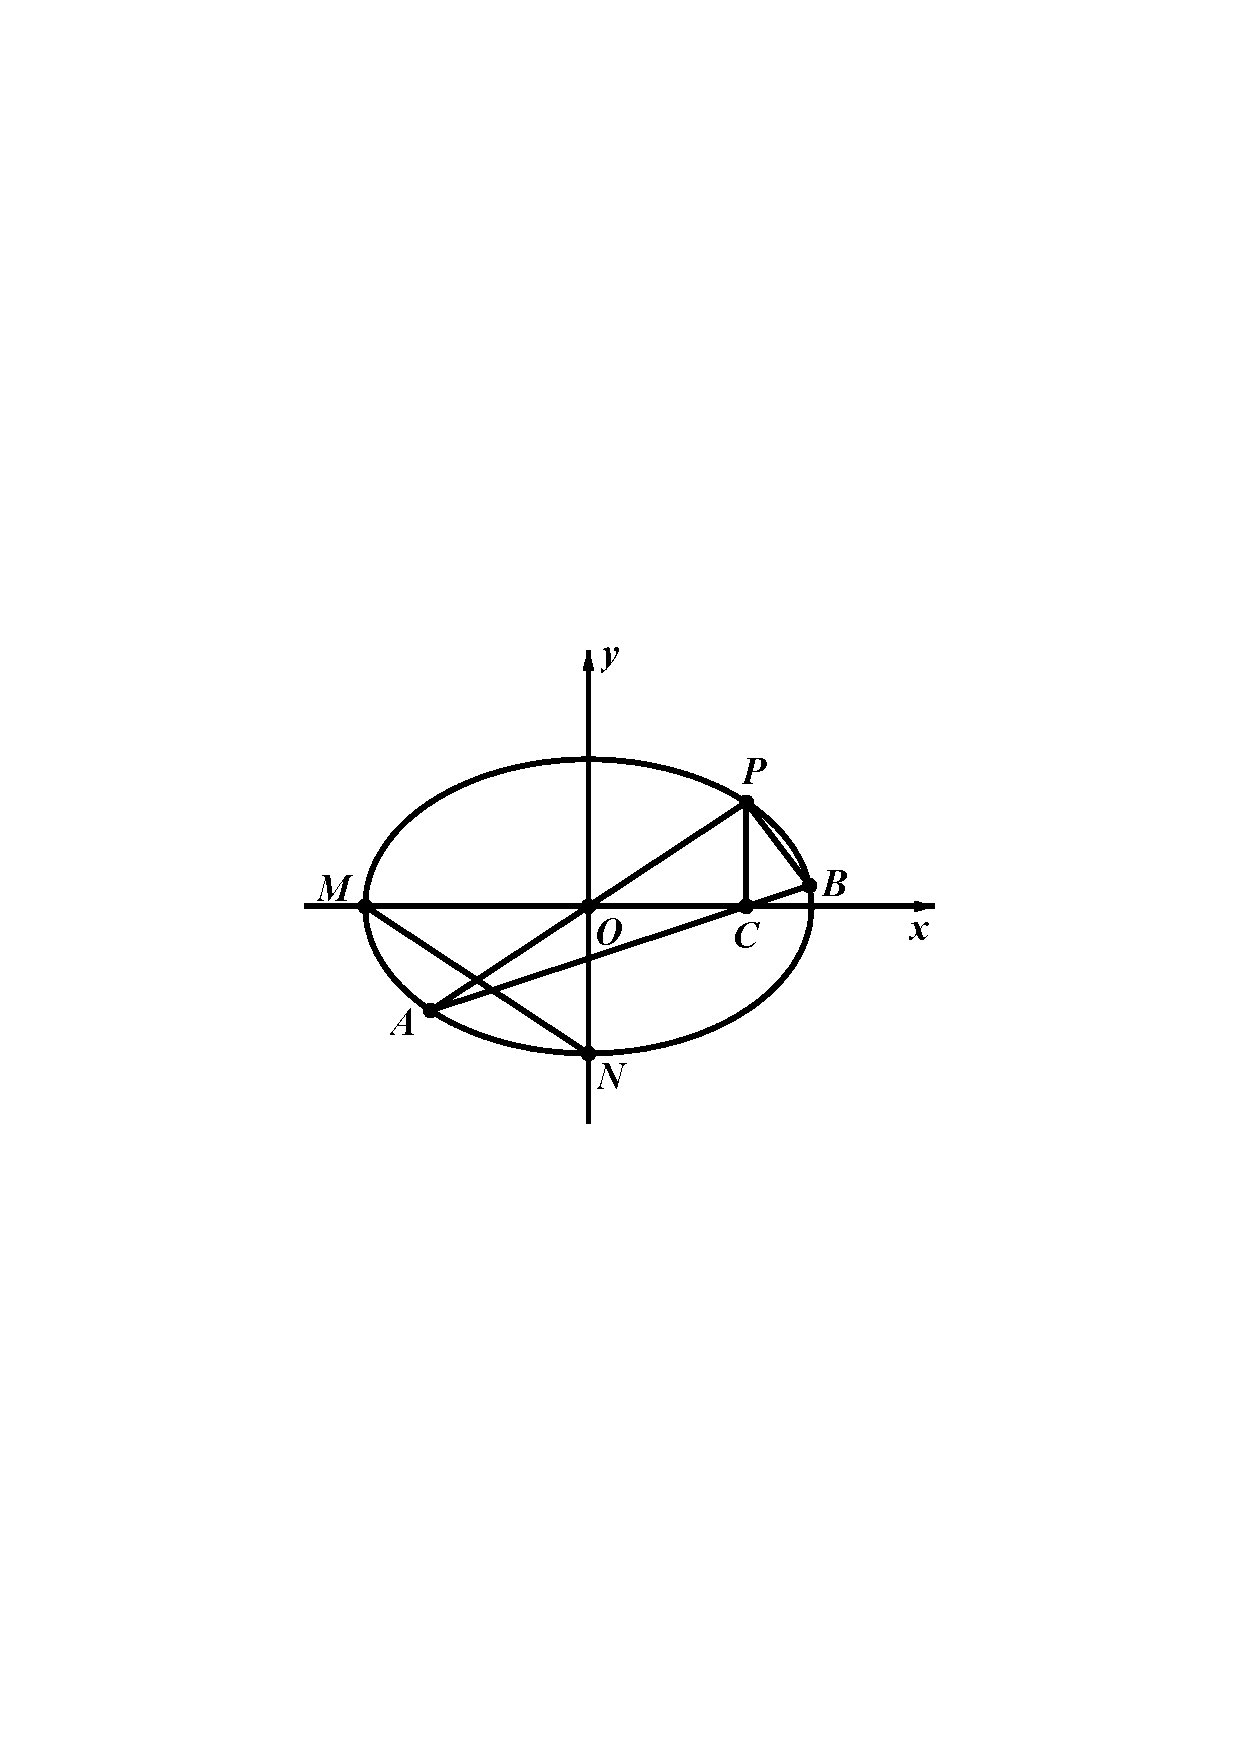
\includegraphics[height=3cm,angle=0]{figs/wangyang_2}\\
%%\caption{椭圆}\label{fig:1}
%\end{center}}
%\end{example}

\begin{example}[2010，重庆卷]
例题的内容$\langle ID,\mu,\gamma\rangle$，$\langle ID,\mu,\gamma\rangle$。
\end{example}
\begin{solution}
解答的内容。
\end{solution}
\begin{exercise}
练习题的内容。
\end{exercise}
\begin{note}
设
\[
D =
\begin{vmatrix}
  5 & 1 & -1 \\
  -7 & 1 & 15 \\
  8 & 1 & -21 \\
\end{vmatrix}
\]
则$D$的第$3$列元的代数余子式的和是$0$。
\end{note}
\begin{proposition}
计算$\displaystyle\int_0^1 \dfrac{x}{\sqrt{1-x^2}} {\rm d}x$。
\end{proposition}
\begin{solution}
因为
$$\int_0^u\frac{x}{\sqrt{1-x^2}} {\rm d}x = -\int_0^u\frac{ {\rm d}(1-x^2)}{2\sqrt{1-x^2}} = \left.-\sqrt{1-x^2}\right|_0^u = 1-\sqrt{1-u^2},$$
所以$\displaystyle\int_0^u\frac{x}{\sqrt{1-x^2}} {\rm d}x = \lim_{u\rightarrow 1^{-}}\int_0^u\frac{x}{\sqrt{1-x^2}} {\rm d}x = 1$。
\end{solution}
\section{矩阵的排版}
分块矩阵的排版示例如下：
\[
\left[
\begin{array}{cc:cc}
a_{11} & a_{12} & b_{11} & b_{12}\\
a_{21} & a_{22} & b_{21} & b_{22}\\
\hdashline
c_{11} & c_{12} & d_{11} & d_{12}\\
c_{11} & c_{12} & d_{11} & d_{12}\\
\end{array}
\right]
\]
\[\mathbf{A} =
\bordermatrix{
      & n_1             & n_2             & \cdots & n_l \cr
  s_1 & \mathbf{A}_{11} & \mathbf{A}_{12} & \cdots & \mathbf{A}_{1l}\cr
  s_2 & \mathbf{A}_{21} & \mathbf{A}_{22} & \cdots & \mathbf{A}_{2l}\cr
  \vdots & \vdots       &        \vdots   &        & \vdots \cr
  s_t & \mathbf{A}_{t1} & \mathbf{A}_{t2} & \cdots & \mathbf{A}_{tl}\cr
}
\]
%A = \begin{pmat}[{..|..}]
%a_{11} & a_{12} & a_{13} & a_{14} & a_{15}\cr
%a_{21} & a_{22} & a_{23} & a_{24} & a_{25}\cr\-
%a_{31} & a_{32} & a_{33} & a_{34} & a_{35}\cr
%\end{pmat},
%$$
\section{算法的排版}
用~\LaTeX{} 可以排出版面非常漂亮的算法\index{算法的排版}。根据所用宏包\index{宏包}的不同，所用的命令也有所不同。下面是用宏包~{\tt algorithm} 和~{\tt algorithmic} 进行算法排版的一个例子。所排的算法是著名的\index{欧几里得算法}欧几里得算法\citeu{stinson}。

%%%%%%%%%%%%%%%%%%%%%%%%%%%%%%%%%%%%%%%%%%%%%%%
\begin{algorithm}
\caption{Euclidean algorithm$(a,b)$}
\label{alg:euclid}
\algsetup{indent=2em}
\begin{algorithmic}[1]
\REQUIRE 整数$a,b\ne 0$
\ENSURE  商序列$q_1,q_2,\cdots,q_m$和$\gcd(a,b)$
\STATE $r_0 \leftarrow a$
\STATE $r_1 \leftarrow b$
\STATE $m\leftarrow 1$
\WHILE{$r_m\ne 0$}
\STATE $q_m\leftarrow\lfloor\frac{r_{m-1}}{r_m}\rfloor$
\STATE $r_m\leftarrow r_{m-1}-q_mr_m$
\STATE $m\leftarrow m+1$
\ENDWHILE
\STATE $m\leftarrow m-1$
\RETURN {$(q_1,q_2,\cdots, q_m;r_m)$}
\STATE {\bf{comment：}$r_m = \gcd(a,b)$ }
\end{algorithmic}
\end{algorithm}
算法~\ref{alg:euclid_no} 是另一个标号\index{算法标号}的。
\begin{algorithm}
\caption{Euclidean algorithm$(a,b)$}
\label{alg:euclid_no}
\algsetup{indent=2em}
\begin{algorithmic}[2]
\REQUIRE 整数$a,b\ne 0$
\ENSURE  商序列$q_1,q_2,\cdots,q_m$和$\gcd(a,b)$
\STATE $r_0 \leftarrow a$
\STATE $r_1 \leftarrow b$
\STATE $m\leftarrow 1$
\WHILE{$r_m\ne 0$}
\STATE $q_m\leftarrow\lfloor\frac{r_{m-1}}{r_m}\rfloor$
\STATE $r_m\leftarrow r_{m-1}-q_mr_m$
\STATE $m\leftarrow m+1$
\ENDWHILE
\STATE $m\leftarrow m-1$
\RETURN {$(q_1,q_2,\cdots, q_m;r_m)$}
%\STATE {\bf{comment：}$r_m = \gcd(a,b)$ }
\end{algorithmic}
\end{algorithm}

%\setcounter{algorithm}{4}
下面的算法~\ref{alg:rgg} 是一个生成$q$进制$n$元反射Gray码\index{反射Gray码}的算法。
\begin{algorithm}
\caption{\sc Reflected Gray Code Generation$(q, n)$}
\label{alg:genGraycode}
\algsetup{indent=2em}
\begin{algorithmic}
%%\TitleOfAlgo{Euclidean algorithm$(a,b)$}
\label{alg:rgg}
\REQUIRE{整数$q>0,n > 0$}
\ENSURE {$q^n\times n$矩阵$G$}
\STATE $g_{n-1}g_{n-2}\cdots g_{0}\longleftarrow 00\cdots 0$
\WHILE{$(2\mid q$ \AND $g_{n-1},g_{n-2},\cdots ,g_{0} \neq q-1,\bm{0}_{n-1})$ \OR $(2\nmid q$ \AND $g_{n-1},\cdots ,g_{n} \neq \bm{(q-1)}_{n}$}
    \STATE $i\leftarrow 0$
    \STATE $\sigma \leftarrow (g_{n-1}+g_{n-2}+\cdots +g_{i+1})\bmod 2$
    \IF{$\sigma=0$ \AND $g_{i}\neq q-1$}
        \STATE $g_{i} \leftarrow g_{i}+1$
    \ELSIF{$\sigma =1$ \AND $g_{i}\neq 0$}
        \STATE $g_{i}\leftarrow g_{i}-1$
    \ENDIF
    \STATE $i \leftarrow i+1$
    \IF{$i = q-1$}
        \STATE $g_{i} \leftarrow g_{i}+1$
    \ENDIF
\ENDWHILE
\end{algorithmic}
\end{algorithm}
%再来一个不标号不连线的：
%\LinesNotNumbered
%\SetAlgoNoLine
%
%\begin{procedure}[H]
%\caption{$f$()\hspace{-.15cm}$(x,a,b)$}
%\label{proc:f}
%\KwIn{$x,a,b$}
%\uIf{$x\in S_1$}{
%    $f\leftarrow (\beta x,a,(b+1)\bmod n)$
%    }
%\uElseIf{$x\in S_2$}{
%    $f\leftarrow (x^2,2a\bmod n,2b\bmod n)$
%    }
%\Else{
%    $f\leftarrow (\alpha x,(a+1)\bmod n,b)$
%    }
%\Return{$(f)$}
%\end{procedure}
\begin{algorithm}
%\COMMENT{external}% {\bf  External: }}
%\begin{algorithmic}
\caption{{\sc Collision-To-Second-Preimage}\,$(h)$}
\label{algo:c2sec}
\begin{algorithmic}
%\REQUIRE{Hash 函数$h$}
\STATE \bf{External: }{\sc Oracle-2nd-Preimage}
\STATE Choose $x\in_R\mathcal{X}$
\IF{{\sc Oracle-2nd-Preimage}\,$(h,x) = x'$}
    \RETURN $(x,x')$
\ELSE{\RETURN{{\rm(``failure")}}}
\ENDIF
\end{algorithmic}
\end{algorithm}

% !TeX TS-program = xelatex
% !Mode TeXUTF-8
%# -- codingutf-8 --
% !TeX encoding = UTF-8
%%%%%%%%%%%%%%%%%%%%%%%%%%%%%%%%%%%%%%%%%%

\zihao{-4}
%---------------------------------------
\chapter{正定矩阵的判定方法}\label{sec:ssss}
%---------------------------------------
我们知道，在高等代数的实际应用以及计算里面，如果能够判定一个矩阵是正定矩阵，往往会给计算带来极大的便利，本章在前面一章的基础上，
总结正定矩阵的判定方法，并借助例题进一步加深对正定矩阵的理解。
\section{定义法}
%----------------------
证明一个矩阵是否为正定矩阵最直接的方法便是验证该矩阵是否满足正定矩阵的定义。然而简单的方法往往只适用于比较简单，条件较少的题型。
就例如例~\eqref{eg:1}，~\eqref{eg:2}
\begin{example}\label{eg:1}\citeu{gaodai_1}
  如果$A$,$B$都是$n$阶的正定矩阵，证明：$A+B$也是正定矩阵
\end{example}
\begin{solution}
  因为$A$,$B$都是$n$阶正定矩阵，所以任意一组不为零的向量$X \in R^{n \times 1}$,都有$X^TAX>0$,$X^TB>0$.又$X^T(A+B)X=X^TAX+X^TBX$,所以$X^T(A+B)X>0$,
  所以$A+B$是正定矩阵。
\end{solution}
\begin{example}(改自华南理工大学2011年研究生考试高等代数试题)\label{eg:2}\citeu{gaodai_2}
  设$A=(a_ij)_{n \times n}$,$B=(b_ij)_{n \times n}$为两个实对称正定矩阵.证明：$n$阶实方阵
  \[C=
\begin{pmatrix}
  a_{11}b_{11} & a_{12}b_{12} & \cdots & a_{1n}b_{1n}\\
  a_{21}b_{21} & a_{22}b_{22} & \cdots & a_{2n}b_{2n}\\
  \vdots & \vdots &            & vdots\\
  a_{n1}b_{n1} & a_{n2}b_{n2} & \cdots & a_{nn}b_{nn}
\end{pmatrix}  
  \]也是正定的
\end{example}
\begin{solution}
   因为$B$是正定矩阵，所以存在可逆矩阵$G$，使得$B=G^TG$,令$G=(g_{ij})$,则$$b_{ij}=\sum_{k=1}^{n} g_{ki}g_{kj}$$
   任取$x=(x_1,x_2,\cdots,x_n)^T \in \mathbb{R}^n$,都有$$x^TCx=\sum_{i=1}^{n} \sum_{j=1}^{n} a_{ij}b_{ij}x_ix_j=
   \sum_{k=1}^{n}(\sum_{i=1}^n \sum_{j=1}^{n} a_{ij}(g_{ki}x_i)(g_{kj}x_j))=\sum_{k=1}^{n}\alpha_k^{T}A\alpha_k$$
   其中$\alpha_k=(g_{k1}x_1,g_{k2}x_2,\cdots,g_{kn}x_n)^T$.因为$A$是正定矩阵，所以$\alpha_k^{T}A\alpha_k>0$,从而
   $$\sum_{k=1}^{n}\alpha_k^{T}A\alpha_k>0$$,既$x^TCx>0$,所以$C$是正定矩阵。
\end{solution}
\section{顺序主子式法}
通过对正定矩阵的分析，我们知道各阶顺序主子式的值均大于零的矩阵是正定矩阵，这种方法在矩阵是低阶尤其是二，三阶的时候格外的好用，但与之
相对应的，在高阶矩阵中，这种方法可以说是毫无用武之地。
\begin{minipage}[t][6cm]{15cm}
  盒子测试。表题应写在表格上方正中，表序写在表题左方不加标点，
  空一格写表题，表题末尾不加标点，全文的表格统一编序，表序必须连续。表题用五号宋体居中，表格内中文用五号宋体，英文用五号Times New Roman字体。

表题允许下页接写，接写时表题省略，表头应重复书写，并在右上方写``续表xx"。下面是一些表格的实例。
\end{minipage}

%\tabulinesep=1.6mm
%
%\begin{tabu} {|X[c]|X[c]|X[c]|X[c]|X[c]|X[c]|X[c]|X[c]|X[c]|X[c]|X[c]|X[c]|X[c]|X[c]|X[c]|X[c]|X[c]|X[c]|X[c]|X[c]|X[c]|X[c]|X[c]|X[c]|X[c]|X[c]|X[c]|X[c]|}
%    \tabucline-
%    \multicolumn{16}{|c}{\raisebox{-1ex}{\zihao{4}{2020}\;学年~第{ \bf 1 }学期}} & \multicolumn{12}{|c|}{\raisebox{-1ex}{\zihao{4}期末考试}}\\\tabucline-
%    \multicolumn{4}{|c}{\bf 考试时间} & \multicolumn{4}{|c}{120分钟} & \multicolumn{4}{|c}{\bf 考核方式} & \multicolumn{5}{|c}{闭卷} & \multicolumn{4}{|c|}{\bf 学生类别} &  \multicolumn{2}{c|}{本科} & \multicolumn{2}{c|}{\bf 人数} & \multicolumn{3}{c|}{100} \\\tabucline-
%    \multicolumn{7}{|c|}{\bf 适用专业或科类} & \multicolumn{14}{c|}{数学 } &  \multicolumn{2}{c|}{{\bf 年级}} & \multicolumn{5}{c|}{2017} \\\tabucline-
%    \tabuphantomline
%\end{tabu}


%\taburulecolor | lime | {blue}
%\arrayrulewidth=1mm \doublerulesep=2mm
%Here is
%\begin{tabu}spread 0pt {X[-1]}
%    \tabucline[\hbox{$\scriptstyle\star$}]
%    a tabu\\
%    environment \\
%    made with \\ \lastline[5mm]\hline\hline\hline
%\end{tabu}TabU package !\par
%And the next paragraph follows
%\begin{tabular}{|>{\bfseries}>{ before }l<{ one } <{ two }|}
%    cell content
%\end{tabular}
%\begin{tabu}to .6\linewidth{cX[2mc]X} \tabucline[1pt]-
%\everyrow{\tabucline[on 2pt ]-}
%This is & a small example & of a \text{tabu} \\
%which   & automatically   & inserts \\
%a horizontal & line after & each of its row \everyrow{} \\ \tabucline[1pt]-
%\end{tabu}

表题应写在表格\index{表格}上方正中，表序写在表题左方不加标点，空一格写表题，表题末尾不加标点，全文的表格统一编序，表序必须连续。
\begin{table}[h]
  \centering
  \caption{一些数学符号的{\LaTeX}输入命令与效果对照表}\label{table:1}
  \begin{tabular}{|c|c|}\hline
  输入 & 输出 \\\hline
  \verb=$(\sum x_{ij})^{1/p}$= & $(\sum x_{ij})^{1/p}$ \\\hline
  \verb=$\left(\sum x_{ij}\right)^{1/p}$= & $\left(\sum x_{ij}\right)^{1/p}$ \\\hline
  \verb=$\bigl(\sum x_{ij}\bigr)^{1/p}$= & $\bigl(\sum x_{ij}\bigr)^{1/p}$ \\\hline
  \verb=$\Bigl(\sum x_{ij}\Bigr)^{1/p}$= & $\Bigl(\sum x_{ij}\Bigr)^{1/p}$ \\\hline
  \verb=$\biggl(\sum x_{ij}\biggr)^{1/p}$= & $\biggl(\sum x_{ij}\biggr)^{1/p}$ \\\hline
  \verb=$\Biggl(\sum x_{ij}\Biggr)^{1/p}$= & $\Biggl(\sum x_{ij}\Biggr)^{1/p}$ \\
  \hline
\end{tabular}
\end{table}
表题用五号宋体居中(见表~\ref{table:1})，表格内中文用五号宋体，英文用五号Times New Roman字体。

表题允许下页接写，接写时表题省略，表头应重复书写，并在右上方写``续表xx"。下面是一些表格的实例。
%\begin{table}
%\tbl{Radio-band beaming model parameters for\\ {FSRQs and BL Lacs.}}
%{\begin{tabular}[l]{@{}lcccccc}
%\toprule
%  Class$^{\rm a}$ & $\gamma _1$ & $\gamma _2$$^{\rm b}$
%
%         & $\langle \gamma \rangle$
%
%         & $G$ & $|{\bm f}|$ & $\theta _{c}$ \\
%
%\hline%colorrule
%  BL Lacs &5 & 36 & 7 & $-4.0$ & $1.0\times 10^{-2}$ & 10$^\circ$ \\
%  FSRQs & 5 & 40 & 11 & $-2.3$ & $0.5\times 10^{-2}$ & 14$^\circ$ \\
%\bottomrule
%\end{tabular}}
%\tabnote{$^{\rm a}$This footnote shows what footnote symbols to use.}
%\tabnote{$^{\rm b}$This footnote shows the text turning over when a long footnote is added.}
%\label{symbols}
%\end{table}

%\taburulecolor | gray!50|{red} \arrayrulewidth=1pt
%{
%\taburulecolor | yellow |{blue}
%\begin{tabu}{|X|X|} \hline
%Here the lines & are drawn in blue \\ \taburulecolor {green} \hline
%But starting from here & they are green coloured ! \\ \hline
%And now a nested tabu & \begin{tabu}{X} \firsthline\hline
%guess what colour \\ \hline
%is used for rules ?\\ \lasthline \hline
%\end{tabu} \\\hline
%\end{tabu}
%In side the group, rule colors are blue
%}%
%After the group, rule colors are red again !
%\begin{tabu}{X}\hline \hline \indent \end{tabu}


\begin{table}[htb]
 \centering\caption{三线表\index{三线表}示例}
\begin{tabular}{ccccc}\toprule
姓名 & 平时成绩 & 期中考试 & 期末考试 & 最后成绩\\\midrule
张三 & 60       & 78       & 76       & 67      \\
李四 & 89       & 92       & 98       & 95      \\
王五 & 95       & 91       & 100      & 97      \\\bottomrule
\end{tabular}
\end{table}
\begin{center}
\begin{tabular}{|c|c|c|c|c|c|c|c|}\hline
\multirow{2}*{题号} & \multicolumn{5}{c|}{第一部分} & \multirow{2}*{第二部分} & \multirow{2}*{总分}\\\cline{2-6}
                    & 一 & 二 & 三 & 四 & 五        &                         & \\\hline
               得分 &    &    &    &    & $\surd$   &                         & \\\hline
\end{tabular}
\end{center}
%\begin{table}[htb]
% \centering
% \caption{一班课程表}
%   \begin{tabular}{|c| *{7}{c|}}\hline
%   \backslashbox{课节}{星期} & 星期一 & 星期二 & 星期三 & 星期四 & 星期五 & 星期六 & 星期日 \\\hline
%   1 & & & & & & &  \\\hline
%   2 & & & & & & &  \\\hline
%   3 & & & & & & &  \\\hline
%   4 & & & & & & &  \\\hline
%   5 & & & & & & &  \\\hline
%   中午& \multicolumn{7}{c|}{}   \\\hline
%   6 & & & & & & &  \\\hline
%   7 & & & & & & &  \\\hline
%   \end{tabular}
%\end{table}
\begin{table}[htb]
\centering
  \begin{tabular}{cc}
   %\caption{左图}
    \begin{tabular}{|ccc|}
      \multicolumn{3}{c}{左表}\\\hline
      a & b & c \\\hline
      d & e & f \\\hline
    \end{tabular}
    &
    %\caption{右图}
    \begin{tabular}{|ccc|}
    \multicolumn{3}{c}{右表}\\\hline
      w  & x  & y  \\\hline
      z  & u  & v  \\\hline
    \end{tabular}\\
  \end{tabular}
\end{table}
%---------------------------------------
\section{公式}
%---------------------------------------
公式应另起一行，正文中的公式\index{公式}、算式或方程式等应编排序号，公式的编号用圆括号括起，
序号标注于该式所在行(当有续行时，应标注于最后一行)的行末。公式可按章节顺序编号或按全文统一编号。公式序号必须连续，不得重复或跳缺。重复引用的公式不得另编新序号。
较长的公式，如必须转行时，最好在等号处转行，如做不到这一点，要在$+,
-, \times, \div$等数学符号处转行。
数学符号应写在转行处的行首。上下式尽可能在等号``="处对齐。
\begin{flushleft}
$
\begin{aligned}
  f(x,y) &= f(0,0) + \frac{1}{1!}\left(x\frac{\partial}{\partial x}+y\frac{\partial}{\partial y}\right)f(0,0) \\
         &= \frac{1}{2!}\left(x\frac{\partial}{\partial x}+y\frac{\partial}{\partial y}\right)^2f(0,0) + \cdots\\
         &= \frac{1}{n!}\left(x\frac{\partial}{\partial x}+y\frac{\partial}{\partial y}\right)^nf(0,0) + K
\end{aligned}
$
\end{flushleft}

\[
\begin{aligned}
f(x,y) &= f(0,0) + \frac{1}{1!}\left(x\frac{\partial}{\partial x}+y\frac{\partial}{\partial y}\right)f(0,0) \\
       &= \frac{1}{2!}\left(x\frac{\partial}{\partial x}+y\frac{\partial}{\partial y}\right)^2f(0,0) + \cdots\\
       &= \frac{1}{n!}\left(x\frac{\partial}{\partial x}+y\frac{\partial}{\partial y}\right)^nf(0,0) + K
\end{aligned}
\]
\begin{equation}\label{eq:a}
    \begin{split}
      f(x,y) =& f(0,0) + \frac{1}{1!}\left(x\frac{\partial}{\partial x}+y\frac{\partial}{\partial y}\right)f(0,0) \\
              & + \frac{1}{2!}\left(x\frac{\partial}{\partial x}+y\frac{\partial}{\partial y}\right)^2f(0,0) + \cdots\\
              & + \frac{1}{n!}\left(x\frac{\partial}{\partial x}+y\frac{\partial}{\partial y}\right)^nf(0,0) + K
    \end{split}
\end{equation}
\[ \Set{x\in\mathbf{R} | 0<|x|<\frac{5}{3}} \]
\[
\left\{\vphantom{\frac{5}{3}}x\in\mathbf{R} \right/\left.
0<{|x|}<\frac{5}{3}\right \}
\]
$$S = \sum_{i=1}^n m_i, \int_a^bf(x)dx = F(x)$$

\[\left\{
\begin{aligned}
  a_{11}x + a_{12}y &= b_1 \\
  a_{21}x + a_{22}y &= b_2
\end{aligned}
\right.
\]
方程组只要一个编号
\begin{equation}
\begin{aligned}
  a_{11}x + a_{12}y &= b_1 \\
  a_{21}x + a_{22}y &= b_2\\
  a_{21}x + a_{22}y &= b_2
\end{aligned}
\end{equation}
或者
\begin{equation}
\left\{
\begin{aligned}
  a_{11}x + a_{12}y &= b_1 \\
  a_{21}x + a_{22}y &= b_2
\end{aligned}
\right.
\end{equation}
方程组中如每个方程要单独编号，则可写成
\begin{numcases}{}
%要使用cases package
        a_{11}x + a_{12}y = b_1\label{eq:111} \\
        a_{21}x + a_{22}y = b_2\label{eq:222}
\end{numcases}
\eqref{eq:111}-\eqref{eq:222}
或
\begin{align}
        a_{11}x + a_{12}y &= b_1 \\
        a_{21}x + a_{22}y &= b_2
\end{align}

\[
f(x) =  \left\{
  \begin{array}{ll}
    x+1, & \hbox{if $x>1$;} \\
    -x, & \hbox{if $x\leq 1$.}
  \end{array}
\right.
\]
\begin{eqnarray}
% \nonumber to remove numbering (before each equation)
  a_{11}x + a_{12}y &=& c_1 \\
  a_{21}x + a_{22}y &=& c_2
\end{eqnarray}
%---------------------------------------
\makeatother
\section{插图}
%\setcounter{totalnumber}{5} 
每幅插图\index{插图}应有图序和图题，全文插图可以统一编序，图序必须连续，不得重复或跳缺。
图序和图题写在图的下方(见图~\ref{fig:1})，五号宋体居中。
\begin{figure}[h]
\centering

\includegraphics[height=6.6cm,angle=0]{preample/ms}\\
\caption{数学与统计学院院徽}\label{fig:1}
\end{figure}
下面是两种图片并列（图~\ref{fig:33} 和图~\ref{fig:44}，图~\ref{fig:21}和图~\ref{fig:22}）的两种情形：
\begin{figure}[h]
\centering
\begin{minipage}[t]{5cm}
\centering
\mbox{\resizebox{!}{35mm}{
\includegraphics{preample/ms}}}\\
\caption{数学与统计学院院徽}\label{fig:33}
\end{minipage}
\hspace{1.5cm}
\begin{minipage}[t]{5cm}
\centering
 \mbox{\resizebox{!}{15mm}{
\includegraphics{preample/xishi}}}\\
 \caption{西南大学校徽字体}\label{fig:44}
\end{minipage}
\end{figure}

%%%%%%%%%%%%%%%%%%%%%%%%%%%%%%%%
\begin{figure}[h]
\centering
\mbox{\subfigure[第一个子图]{\resizebox{!}{15mm}{

\includegraphics{preample/xishi}\label{fig:21}
}}}\hspace{1.5cm}
\mbox{\subfigure[第二个子图]{\resizebox{!}{35mm}{

\includegraphics{preample/ms}\label{fig:22}
}}}\\
\caption{西南大学与数学与统计学院}
\end{figure}

% !TeX TS-program = xelatex
% !Mode TeXUTF-8
%# -- codingutf-8 --
% !TeX encoding = UTF-8
%%%%%%%%%%%%%%%%%%%%%%%%%%%%%%%%%%%%%%%%%%

\large\zihao{-4}
%---------------------------------------
\chapter{正定矩阵的解题应用}\label{sec_si4}
%---------------------------------------
在高等代数中，正定矩阵对于解决难题扮演着重要的角色。本章主要内容是通过例题来介绍正定矩阵在高等代数解题中的几种应用。
\section{矩阵分解}
正定矩阵作为矩阵的一种特殊形式，最直接的应用就是可以将矩阵分解。与正定矩阵相关的矩阵分解定理有很多，下面列举几个作为例子：
\begin{enumerate}
    \item 矩阵的极分解：若$A$是一个$n$阶实可逆矩阵，则存在一个正交矩阵$U$和正定矩阵$P$使得$A=PU$且该分解是唯一的;
    \item \textit{Cholesky}分解：若$A$是$n$阶正定矩阵，则存在一个对角元为正数的上三角矩阵$R$，使得$A=R^\mathrm{T}R$,且该分解是唯一的；
    \item 若$A$是$n$阶正定矩阵，则存在一个正定矩阵$C$使得$A=C^2$
\end{enumerate}
\begin{example}
    设$A$是$n$阶正定矩阵，证明：$A$的所有顺序主子式均大于零，当且仅当存在唯一的对角元全为1的上三角矩阵$S$和对角元全为正的对角矩阵$D$，
    使得$A = S^\mathrm{T} D S$。
\end{example}
\begin{solution}
必要性：若$A$为正定矩阵，则其所有顺序主子式均大于零。
根据Cholesky分解定理，存在唯一的对角元为正数的上三角矩阵$R$，使得
$A = R^\mathrm{T}R$
令对角矩阵
$$D = \operatorname{diag}(r_{11}^2, r_{22}^2, \cdots, r_{nn}^2), \quad r_{ii}>0,$$
构造矩阵
$$S = R \cdot \operatorname{diag}\left(\frac{1}{r_{11}}, \frac{1}{r_{22}}, \cdots, \frac{1}{r_{nn}}\right),$$
则$S$为对角元全为$1$的上三角矩阵，且$R = S\sqrt{D}$。代入Cholesky分解式得：
$$
A = R^\mathrm{T} R = (S\sqrt{D})^\mathrm{T} (S\sqrt{D}) = S^\mathrm{T} D S.
$$
故分解$A = S^\mathrm{T} D S$存在。

下证唯一性：

假设存在两组分解$$A = S_1^\mathrm{T} D_1 S_1 = S_2^\mathrm{T} D_2 S_2,$$
其中$S_1,S_2$为对角元全为1的上三角矩阵，$D_1,D_2$为对角元全为正的对角矩阵。

整理得$$(S_2^\mathrm{T})^{-1}S_1^\mathrm{T} D_1 = D_2 S_2 S_1^{-1}.$$
左边是下三角矩阵，右边是上三角矩阵，因此两边均为对角矩阵。
结合$S_1,S_2$对角元为1，可得$S_1 = S_2$，进而$D_1 = D_2$，分解唯一。

充分性：
若存在分解$A = S^\mathrm{T} D S$，其中$S$为对角元全为1的上三角矩阵（可逆），$D = \operatorname{diag}(d_1,d_2,\cdots,d_n),d_i>0$。
对任意非零向量$x \in \mathbb{R}^n$，令$y = Sx$，则$y \neq 0$，且
$$
x^\mathrm{T} A x = x^\mathrm{T} S^\mathrm{T} D S x = y^\mathrm{T} D y = \sum_{i=1}^n d_i y_i^2 > 0.
$$
故$A$为正定矩阵，其所有顺序主子式均大于零。

综上，命题得证
\end{solution}

\section{不等式}
根据正定矩阵的定义，我们可以知道，正定矩阵与不等式有着紧密的联系。关于正定矩阵的不等式有很多，要证明这些不等式就要综合的运用正定矩阵的性质、
定理、判定方法等。
\begin{example}\citeu{gaodai_1}
    设$A=(a_{ij})$是$n$阶正定矩阵，证明：\begin{enumerate}
        \item $|A|\leqslant a_{nn}H_{n-1}$,$H_{n-1}$是$A$的$n-1$阶顺序主子式
        \item $|A|\leqslant a_{11}a_{22}\cdots a_{nn}$
    \end{enumerate}
\end{example}
\begin{solution}
    (1)将矩阵 $A$ 进行分块如下：
\[
A = \begin{pmatrix} A_{n-1} & \alpha \\ \alpha^\mathrm{T} & a_{nn} \end{pmatrix}
\]
其中 $A_{n-1}$ 是 $A$ 的左上角 $n-1$ 阶子矩阵（即 $n-1$ 阶顺序主子阵），
$\alpha = (a_{1n}, a_{2n}, \cdots, a_{n-1,n})^\mathrm{T}$ 是列向量。因为 $A$ 是正定矩阵，所以其顺序主子阵 $A_{n-1}$ 也是正定的，
故 $A_{n-1}$ 可逆，且 $H_{n-1} = \det(A_{n-1}) > 0$。

构造分块初等矩阵 $P$，对 $A$ 作初等变换：
\[
P = \begin{pmatrix} E_{n-1} & 0 \\ -\alpha^\mathrm{T} A_{n-1}^{-1} & 1 \end{pmatrix},
\text{其中 $E_{n-1}$ 为 $n-1$ 阶单位矩阵.}\]

计算 $P^\mathrm{T} A P$：
\begin{align*}
P^\mathrm{T} A P &= \begin{pmatrix} E_{n-1} & -A_{n-1}^{-1}\alpha \\ 0 & 1 \end{pmatrix} 
\begin{pmatrix} A_{n-1} & \alpha \\ \alpha^\mathrm{T} & a_{nn} \end{pmatrix} 
\begin{pmatrix} E_{n-1} & 0 \\ -\alpha^\mathrm{T} A_{n-1}^{-1} & 1 \end{pmatrix} \\
&= \begin{pmatrix} A_{n-1} & 0 \\ 0 & a_{nn} - \alpha^\mathrm{T} A_{n-1}^{-1}\alpha \end{pmatrix}
\end{align*}
该变换保持行列式的值不变，对两边取行列式：
\[
\det(P^\mathrm{T} A P) = \det(A) = \det(A_{n-1}) \cdot (a_{nn} - \alpha^\mathrm{T} A_{n-1}^{-1}\alpha)
\]
由于 $A$ 正定，对于任意非零向量 $x$，$x^\mathrm{T} A x > 0$。取 $x = A_{n-1}^{-1}\alpha$，
可知 $\alpha^\mathrm{T} A_{n-1}^{-1}\alpha > 0$，因此：
\[
a_{nn} - \alpha^\mathrm{T} A_{n-1}^{-1}\alpha \le a_{nn}
\]
代入行列式公式得：
\[
|A| = H_{n-1} \cdot (a_{nn} - \alpha^\mathrm{T} A_{n-1}^{-1}\alpha) \le H_{n-1} \cdot a_{nn}
\]
即 $|A| \le a_{nn}H_{n-1}$，(1) 得证。

(2)对$A$的阶数$n$做数学归纳法。
当 $n=1$ 时，$|A| = a_{11}$，不等式显然成立。
当 $n=2$ 时，设 $A = \begin{pmatrix} a_{11} & a_{12} \\ a_{21} & a_{22} \end{pmatrix}$，则 $|A| = a_{11}a_{22} - a_{12}^2 \le a_{11}a_{22}$，结论成立。

假设对于任意 $n-1$ 阶正定矩阵，结论成立，即 $n-1$ 阶正定矩阵的行列式小于等于其对角元乘积。

对于 $n$ 阶正定矩阵 $A$，由 (1) 的结论可知：
\[
|A| \le a_{nn} \cdot |A_{n-1}|
\]
其中 $A_{n-1}$ 是 $n-1$ 阶正定矩阵。根据归纳假设：
\[
|A_{n-1}| \le a_{11}a_{22}\cdots a_{n-1,n-1}
\]
因此：
\[
|A| \le a_{nn} \cdot (a_{11}a_{22}\cdots a_{n-1,n-1}) = a_{11}a_{22}\cdots a_{nn}
\]
由数学归纳法原理，不等式对任意正整数 $n$ 成立。
\end{solution}

\section{极值问题}
在数学分析里，我们知道，当$n$元函数$f$若在$x_0$的某个领邻域里存在二阶偏导数，且$f'(x_0)=0$,则当$f$在$x_0$的黑塞(Hesse)矩阵$f''(x)$
是正定矩阵时，$f$在$x_0$处取严格极小值。也就是说我们可以用正定矩阵来求取多元函数的极小值。 
\begin{example}
    求三元函数
\[
f(x,y,z)=x^2 + 2y^2 + z^2 + xy + xz - 3x - 2y - z
\]
的极值。
\end{example}
\begin{solution}

分别求一阶偏导数，并令其为零：
\[
\begin{cases}
f_x = 2x + y + z - 3 = 0\\
f_y = x + 4y - 2 = 0\\
f_z = x + 2z - 1 = 0
\end{cases},\text{解此方程组，得驻点为}
\begin{cases}
    x=\frac{8}{5}\\ y=\frac{1}{10}\\z=-\frac{3}{10}
\end{cases}
\]

求二阶偏导数，得Hessian矩阵：
\[
H =
\begin{pmatrix}
f_{xx} & f_{xy} & f_{xz}\\
f_{yx} & f_{yy} & f_{yz}\\
f_{zx} & f_{zy} & f_{zz}
\end{pmatrix}
=
\begin{pmatrix}
2 & 1 & 1\\
1 & 4 & 0\\
1 & 0 & 2
\end{pmatrix}.
\]

依次计算各阶顺序主子式：
\[
\Delta_1 = 2 > 0,\quad
\Delta_2 = \begin{vmatrix}2 & 1\\1 & 4\end{vmatrix} = 7 > 0,\quad
\Delta_3 = \begin{vmatrix}2 & 1 & 1\\1 & 4 & 0\\1 & 0 & 2\end{vmatrix} = 10 > 0.
\]

故Hessian矩阵 $H$ 为正定矩阵，因此函数 $f(x,y,z)$ 在驻点
\[
\left(\frac{8}{5},\frac{1}{10},-\frac{3}{10}\right)
\]
处取得极小值。
\end{solution}

以上只是正定矩阵在部分领域的应用，而正定矩阵的应用是广泛的，多领域的。除了我所提到的三种，正定矩阵在工程，技术领域、在经济金融领域、
信息技术领域等诸多领域发挥着不可替代的作用。
% !TeX TS-program = xelatex
% !Mode TeXUTF-8
%# -- codingutf-8 --
% !TeX encoding = UTF-8
%%%%%%%%%%%%%%%%%%%%%%%%%%%%%%%%%%%%%%%%%%

\large\zihao{-4}

\chapter{结论}\label{sec:codeinludsion}


%==================参考文献========================
% !TeX TS-program = xelatex
% !Mode TeXUTF-8
%# -- codingutf-8 --
% !TeX encoding = UTF-8
%%%%%%%%%%%%%%%%%%%%%%%%%%%%%%%%%%%%%%%%%%%%%%
\renewcommand{\baselinestretch}{\yuanbeishu}                                                 
\addcontentsline{toc}{chapter}{参考文献}   
%\chapter*{}  
\begin{thebibliography}{99}   \zihao{5}{                 
%%%%%%%%%%%%%%%%%%%%%%%%%%%%%%%%%%%%%%%%%%%%%%
\bibitem{wai_1}
    Horn R A,Johnson C R.
\textsl{Matrix Analysis}[M].New York: Cambridge University Press, Cambridge,1985.
\bibitem{gaodai_1}
北京大学数学系前代数与几何教研室代数小组[王萼芳，石生明 修订]，
\textsl{高等代数（第五版）} [M]. 高等教育出版社，2019年
\bibitem{gaodai_2}
丘维声
\textsl{高等代数(上册)——大学高等代数课程创新教材}[M].北京：清华大学出版社，2010.6

\bibitem{moban_wenjian}
    西南大学.
    \textsl{关于印发《西南大学全日制本科学生毕业论文（设计）工作管理办法》的通知.}
    \href{http://jwc.swu.edu.cn/\_\_local/6/D2/C1/4328A82EE22467E1BE3211788BB\_70028746\_53B64.pdf?e=.pdf}{http://jwc.swu.edu.cn/\_\_local/6/D2/C1/4328A82EE22467E1BE3211788BB\_70028746\_53B64.pdf?e=.pdf}
    
\bibitem{moban_fujian}
西南大学. \emph{西校〔2021〕4号附件.docx}~\href{http://jwc.swu.edu.cn/info/1020/2347.htm}
    {http://jwc.swu.edu.cn/info/1020/2347.htm}
\bibitem{tongzhi}
西南大学数学与统计学院.
\textsl{关于2017届本科毕业论文工作安排的通知}.
\bibitem{experqc}
    C.H.Bennett, F.Bessette, G.Brassard, et al,
    \textsl{Experimental quantum cryptography} [J].
    Journal of Cryptology, Vol.5, No.1(1992), 3--28.
\bibitem{latex}
    \TeX\, Guru.
    \textsl{\LaTeXe 用户手册}. 1999.
\bibitem{knuth}
    Donald E. Knuth,
    \textsl{The \TeX book} [M]. Addison-Wesley, 1984.
\bibitem{knuth_2}
    Donald E. Knuth,
    \textsl{The Arts of Computer Programming} [M]. 北京：机械工业出版社, 2008.
\bibitem{jiaocheng}
    赫尔穆特.科普卡，帕特里克 W. 达利,
    \textsl{\LaTeX 实用教程（英文版第$4$版）}[M]. 北京：机械工业出版社，2005.
\bibitem{latex_hu}
    胡伟,
    \textsl{\LaTeXe 完全学习手册（第二版）}[M]. 北京：清华大学出版社，2013.4.
\bibitem{stinson}
    D. R. Stinson,
    \textsl{Cryptography---Theory and Practice (Third Edition)}[M]. Chapman \& Hall/CRC, Taylor \& Francis Group, Roca Raton, FL, USA. 164.

\bibitem{companion}
    Frank Mittelbach, Michel Goossens.
    \textsl{The \LaTeX \,Companion (Second Edition)}[M]. Addison-Wesley, 2005.
\bibitem{zhanglibo}
    张林波等.
    \textsl{CCT中外文科技排版系统} [M].北京：海洋出版社，1993年。
\bibitem{zhang}
    张禾瑞,
    \textsl{近世代数} [M].高等教育出版社, 1978年.
\bibitem{das}
    Das,M.L., Saxena, A., and Phatak,D.B.
    \emph{Algorithms and Approaches of Proxy Signature: A Servey}. arXiv:cs/0612098v1 [cs.CR],20 Dec 2006. ~\href{https://arxiv.org/pdf/cs/0612098.pdf}{https://arxiv.org/pdf/cs/0612098.pdf.}
\bibitem{xiong}
    熊全淹,
    \textsl{近世代数} [M]. 武汉大学出版社, 1995年.
}
\end{thebibliography}

%====================索引==========================
\printindex %如不要索引请将此行和下行注释掉
\addcontentsline{toc}{chapter}{索引}
%====================致谢==========================
% !TeX TS-program = xelatex
% !Mode TeXUTF-8
%# -- codingutf-8 --
% !TeX encoding = UTF-8
%%%%%%%%%%%%%%%%%%%%%%%%%%%%%%%%%%%%%%%%%%
%%%%%%%%%%%%%%%%%%%%%%%%%%%%%%%%%%%%%%%%%%%%%%%%%%%%%
\renewcommand{\baselinestretch}{\beishu}\normalsize %
%%%%%%%%%%%%%%%%%%%%%%%%%%%%%%%%%%%%%%%%%%%%%%%%%%%%%
%\noindent\large\zihao{-4}{\bf 致谢：}
\CTEXsetup[format+={\flushleft\zihao{4}\ziju{0}}]{chapter}
\addcontentsline{toc}{chapter}{致谢}
\chapter*{致谢：}%\label{endofThesis}
%-----------------------------------
本模板目前的版本是由2006年完成的初始版经多年反复修改而来。西南大学数学与统计学院前后\nianxian 届同学在使用过程中所反馈的意见
是本模板发展的强大推动力。在此我要感谢所有使用过模板的同学，尤其是模板完成后最初几年使用过的同学，他们承受了初期模板中存在的问题所带给他们的种种不便，有时甚至可能是痛苦。同时我也要感谢数学与统计学院的领导和某些老师对使用本模板的宽容态度，
正是由于他们的宽容，才使得本模板的使用和推广成为可能。我还要特别感谢我的同事彭作祥教授多年来的热情鼓励以及一些有益的建议，
他在2014年就将模板推荐给统计系$2015$届的同学使用，从而使更多的同学开始接触到~\LaTeX。早在2016年，学院就`` 建议所有学生的毕业论文（设计）均使用~latex 模板排版"\citeu{tongzhi}。到了2019年，学院就要求所有毕业生使用~\LaTeX 撰写毕业论文，而我本人一直欢迎和鼓励同学们使用我这个模板。

希望大家在使用~\LaTeX{} 编辑完成论文后能体会到当年~D.E.Knuth 教授在修订他的长篇巨著《The Arts of Computer Programming》\cite{knuth_2} 时还不得不抽出大量的时间来设计、
研制~\LaTeX{} 的前身~\TeX{} 的心情，以及~\LaTeX{} 对当今社会的影响。同时我更希望~\LaTeX{} 能给大家今后的工作、学习和生活带来更多的便利。

由于~\LaTeX{} 一直在不断的更新，同时计算机的操作系统也在不断升级，再加上本人也仅仅是一个业余的~\LaTeX{} 爱好者，水平有限，因此模板难免会有这样或那样的问题。请将问题或者建议~email (\href{mailto:xbao@swu.edu.cn}{\tt xbao@swu.edu.cn})告诉我。感谢大家的意见和反馈！

\vspace{2cm}

\begin{center}
    \begin{tabular}{cp{3cm}c}
         &   & {\fangsong \minzi}        \\
         &   & {\fangsong \tijiaoriqi}   \\
         &   & {\fangsong  于\zhixiedizhi}\\
     \end{tabular}
\end{center}

%====================附录==========================
\include{fujian/fulu}%如没有附录，请将这句注释掉
%==================================================
\end{document}
%====END OF PAPER====
